 \newchapter{feedforward}{Best Achieved Phase Stabilisation}

Over the course of 2014 and 2015 much experience has been gained with the PFF system and vast improvements have been made to the system setup, hardware performance and beam conditions as discussed in previous chapters. Many datasets have been taken, in particular in December~2014, July~2015 and November~2015, and in all cases a reduction in downstream phase jitter has been achieved. The purpose of this chapter is to present and discuss the downstream phase stability that was accomplished on the 20th November 2015, the day during which the best overall conditions to date for the PFF correction were obtained.

\newsection{jitterRecord}{Lowest Achieved Phase Jitter}

The results presented in this section show the best downstream phase jitter currently achieved at CTF3 with the PFF correction. Naturally, this dataset was taken during the best beam conditions currently achieved at CTF3 in terms of phase propagation, taken just after a series of R56 and beam energy optimisations using the same methods discussed in Chapter~\ref{c:phasePropagation}. In particular, the first attempt to smooth the upstream phase along the pulse by adjusting the waveform of the first klystron in the CTF3 injector (MKS02) as described in Section \ref{ss:t566Mitigation} yielded the highest upstream-downstream phase correlation achieved to date in normal conditions (higher correlations can be achieved by adding an additional jitter source upstream, as seen in Section~\ref{s:pffNovelSetups}). November~2015 also represents the first time the PFF system was operated with the improved phase monitor resolution after switching to mechanical phase shifters (Section~\ref{s:shifters}) and with the latest version of the amplifier which doubled the correction range compared to earlier tests (Section~\ref{s:amplifierSetup}).
 
The dataset was taken on the 20th November 2015 as one of a sequence of short measurements fine-tuning the gain around the optimal value. Results from the other datasets in this sequence are discussed in the following section to demonstrate the phase stability achieved on longer time scales. The individual dataset shown here comprises 150 pulses taken in interleaved mode, with the correction applied to the 75 odd indexed pulses and no correction applied to the remaining 75 even indexed pulses. The used gain in FONT5a units was 800, corresponding to an actual applied correction of 1.13 times the upstream phase using the conversion factor calculated in Section \ref{ss:fontSetup}



\subsection{Mean Phase Jitter}
\label{ss:bestMeanJitter}

Initially considering the mean pulse phase, the correlation with the PFF correction off in this dataset, as shown by the blue distribution of points in Figure \ref{f:BestFF_Real}, is \(0.93\pm0.04\). This gives a theoretical limit of a factor \(2.7\pm0.4\) reduction in the downstream jitter using Equation \ref{e:theoretJitOptGain}. The achieved uncorrected downstream mean phase jitter of \(0.74\pm0.06^\circ\) and downstream-upstream jitter ratio of \(1.1\pm0.1\) are also the lowest achieved at CTF3 to date. With this initial jitter and the theoretical reduction factor of \(2.7\pm0.4\) the lowest corrected downstream jitter that could be achieved is then \(0.27\pm0.05^\circ\). The aforementioned correlation and jitter ratio combine to give an optimal gain of \(1.0\pm0.1\) (Equation \ref{e:theoretOptGain}). The actual system gain of 1.1 and the optimal gain therefore agree within the error bars, thus the theoretical corrected downstream jitter of \(0.27\pm0.05^\circ\) should also be possible with the actual system.

\begin{figure}
  \centering
  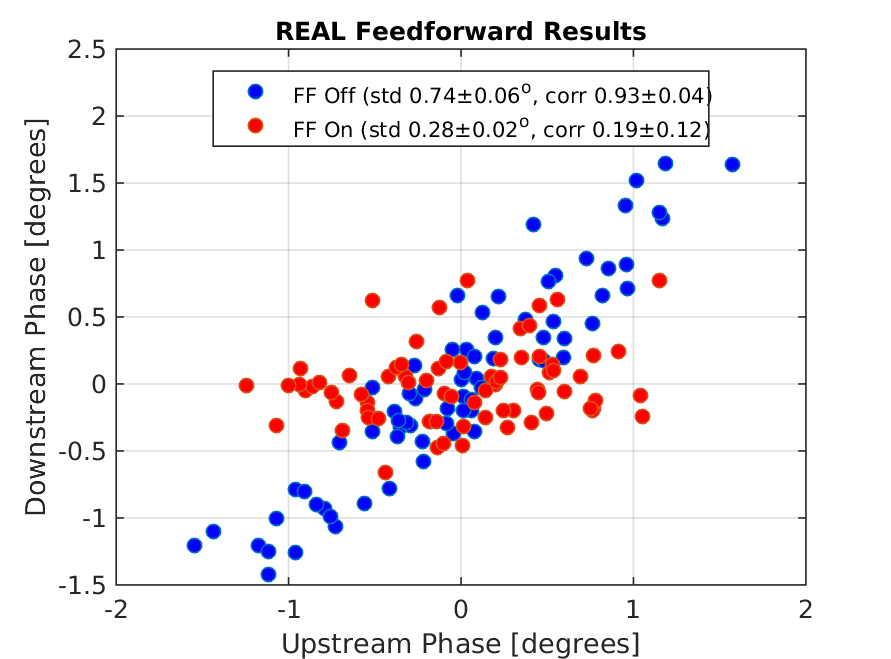
\includegraphics[width=0.75\textwidth]{Figures/feedforward/BestFF_Real}
  \caption{Mean phase.}
  \label{f:BestFF_Real}
\end{figure}

The red distribution of points in Figure \ref{f:BestFF_Real} then shows the effect of the PFF correction on the phase distribution. The downstream phase jitter is reduced from \(0.74\pm0.06^\circ\) to \(0.28\pm0.02^\circ\), a reduction of a factor \(2.6\pm0.3\).  Within the error this does indeed agree perfectly with the theoretical limit derived previously given the beam conditions in this dataset, as expected. The correction acts to remove all correlation between the upstream and downstream phase, rotating the distribution as seen in the plot. The correlation is reduced from \(0.93\pm0.04\) to \(0.19\pm0.12\). 

In terms of the achieved downstream phase jitter it should be noted, however, that the measured upstream jitter of \(0.57\pm0.05^\circ\) across the pulses with the PFF correction on in this dataset is lower than the \(0.69\pm0.06^\circ\) measured with the PFF system off (Table \ref{t:BestFF}). This is assumed to be a statistical fluctuation rather than being a systematic difference between the odd and even pulses at CTF3 or an effect of the correction (which can only influence the downstream phase). Assuming the PFF on upstream jitter propagated downstream with the same ratio as the PFF off data, the true `natural' downstream jitter without the correction applied would have been \(0.61\pm0.09^\circ\) and the true factor reduction in the corrected jitter achieved with the PFF system would be decreased to \(2.2\pm0.4\). Assuming the upstream-downstream phase correlation was also not affected by this statistical fluctuation (so that the theoretical jitter reduction of a factor \(2.7\pm0.4\) still holds), a corrected jitter of \(0.23\pm0.05^\circ\) would have been theoretically possible for the PFF on pulses in this dataset. 

With interleaved data it is also possible to simulate the expected effect of the correction empirically, as an additional point of comparison between the achieved and expected results plus to verify that the complete behaviour of the system is understood. The distribution of simulated corrected phases is shown in green on Figure \ref{f:BestFF_Simulated}. It is derived by taking the initial distribution with the PFF system off (blue points) and subtracting the upstream phase, multiplied by a gain factor, from the downstream phase. This exactly mimics what the feedforward system would have done if it had been applied to the even pulses in this dataset, and can be directly compared to the odd pulses taken at the same time with the actual correction applied. In this example the simulation shown is the ideal case, considering a correction with infinite range and bandwidth applied with the optimal gain. As expected the simulated corrected downstream jitter of \(0.27\pm0.02\) agrees perfectly with the theoretical prediction of \(0.27\pm0.05^\circ\) previously derived. The achieved jitter of \(0.28\pm0.02\) matches both the theoretical and simulated jitter predictions within the error, giving confidence that the overall PFF setup in this dataset (after all the commissioning steps discussed in Chapter \ref{c:commissioning}) was close to optimal. There is perhaps some room for improvement due to the difference between the upstream jitter in the PFF on and off data, as mentioned previously, and this will be elaborated on in Section \ref{s:longPFF} below. Nevertheless, this result clearly demonstrates stability on the mean phase approaching the CLIC target of 0.2 degrees at 12~GHz and demonstrates that achieving this stability with a PFF system is feasible.


\begin{figure}
  \centering
  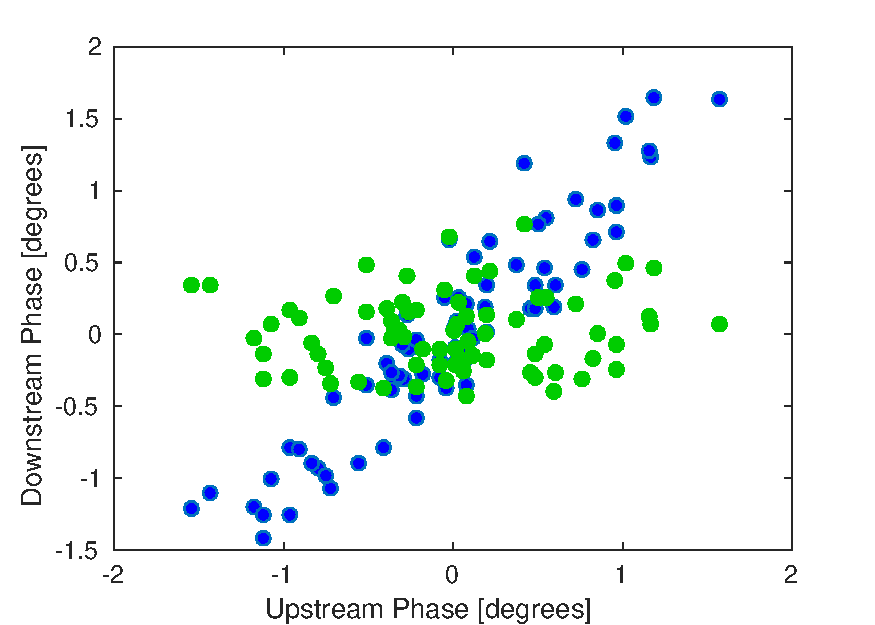
\includegraphics[width=0.75\textwidth]{Figures/feedforward/BestFF_Simulated}
  \caption{Simulated PFF.}
  \label{f:BestFF_Simulated}
\end{figure}


\begin{table}
  \begin{center}
    \begin{tabular}{| c | c | c | c |}
	   \hline
       Correction Status & Upstream Jitter & Downstream Jitter & Correlation \\ \hline
       FF Off & \(0.69\pm0.06^\circ\) & \(0.74\pm0.06^\circ\) & \(0.93\pm0.04\) \\
	   FF On & \(0.57\pm0.05^\circ\) & \(0.28\pm0.02^\circ\) & \(0.19\pm0.12\) \\
	   FF Simulated & \(0.69\pm0.06^\circ\) & \(0.27\pm0.02^\circ\) & \(0.06\pm0.12\) \\ \hline
    \end{tabular}
    \caption{Best PFF results.}
  	\label{t:BestFF}
  \end{center}
\end{table}

\subsection{Correction of Pulse Shape}
\label{ss:bestPulseShape}

Moving on to the stabilisation of the phase along the pulse, Figure~\ref{f:BestFF_MeanPhaseAlong} shows the mean phase along the pulse upstream, downstream with the PFF system off and downstream with the PFF system on. The vertical black lines mark the sample range that was used to calculate the mean phase results presented previously. This range is chosen to cover the maximal proportion of the pulse within which the the correction is not being saturated as a result of the phase sag (plus jitter) exceeding the \(\pm6^\circ\) correction range. It covers a total of 81 samples at 5.2 ns per sample, giving a total time span of 422~ns. The demonstration of \(0.28\pm0.01^\circ\) mean phase stability is therefore already on a much longer pulse than is needed for CLIC, where the combined pulse length is only 240~ns. 

With the optimised phase propagation in place the overall shape of the upstream and (uncorrected) downstream phase, in green and blue respectively, along the pulse are very similar, although small uncorrelated variations are still visible. These uncorrelated differences are then visible in the corrected downstream phase (in red), although the overall ability of the PFF system to flatten the CTF phase sag within the sample range is strikingly clear. The original peak-to-peak variation in the mean downstream phase along the pulse of \(5.76\pm0.14^\circ\) with the correction off is reduced to \(0.65\pm0.07^\circ\) degrees with the correction applied within the indicated range. Outside the central region of the pulse, where the amplifier is saturated, the PFF system can no longer correct the shape of the phase along the pulse. The only effect is to shift the phase by the maximum possible correction of \(5.5^\circ\).

\begin{figure}
  \centering
  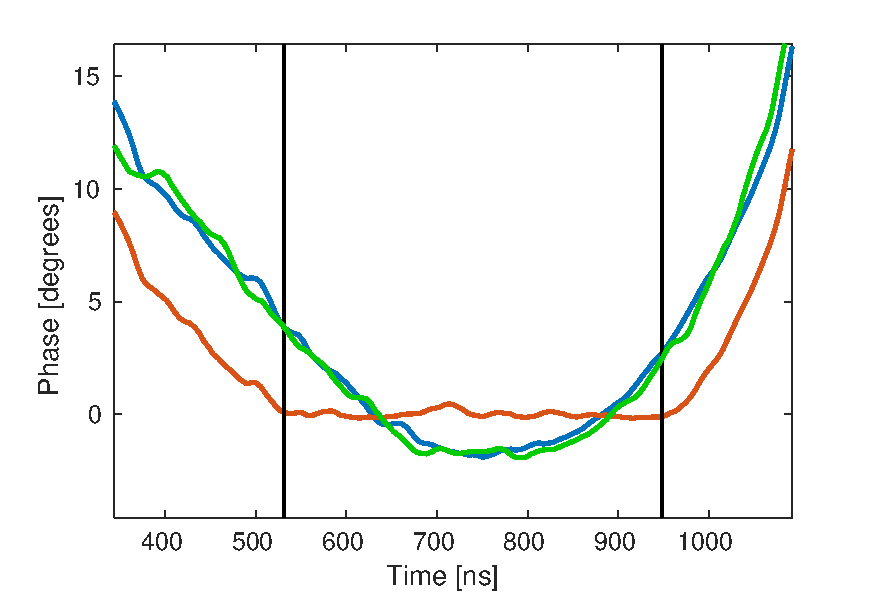
\includegraphics[width=0.75\textwidth]{Figures/feedforward/BestFF_MeanPhaseAlong}
  \caption{Mean phase along.}
  \label{f:BestFF_MeanPhaseAlong}
\end{figure}

Figure \ref{f:BestFF_Flatness} expresses the effect of the PFF system on the phase along the pulse within the central region in terms of the distribution of `flatness' values for each pulse in the data set with PFF system off and on. For each pulse the flatness value is defined as the standard deviation of phase values about the mean across the sample range. In this case the flatness value of each pulse therefore corresponds to the standard deviation of 81 values (the length of the sample range). A pulse with a flatness value of zero would have constant phase across the whole sample range, with no small variations such as those seen in Figure \ref{f:BestFF_MeanPhaseAlong}. The value is also insensitive to the jitter on the overall mean pulse phase seen earlier in Figure \ref{f:BestFF_Real}. In Figure \ref{f:BestFF_Flatness}, the initial uncorrected downstream pulse flatness, dominated by the phase sag at CTF3, of \(1.68\pm0.02^\circ\) is reduced to \(0.26\pm0.01^\circ\) with the correction applied. On average, the corrected pulses are \(6.5\pm0.3\) times `flatter' than the uncorrected pulses.

\begin{figure}
  \centering
  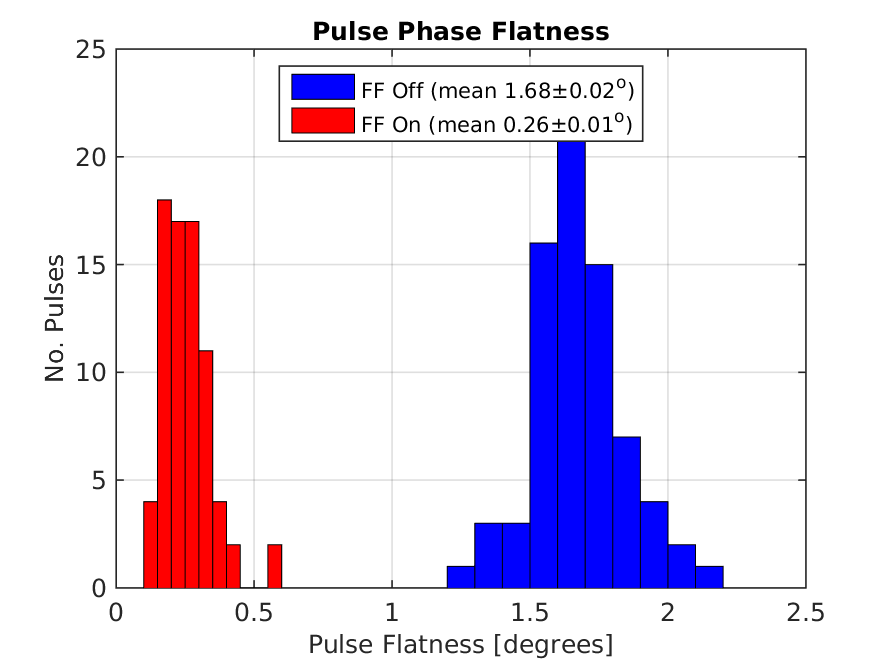
\includegraphics[width=0.75\textwidth]{Figures/feedforward/BestFF_Flatness}
  \caption{Flatness.}
  \label{f:BestFF_Flatness}
\end{figure}

\subsection{Phase Jitter Along the Pulse}
\label{ss:bestJitterAlong}

Finally, Figure \ref{f:BestFF_StdPhaseAlong} shows the overall phase jitter at each sample along the pulse upstream and downstream with the PFF system off and on. These jitter values contain components coming from both the jitter on the overall mean pulse phase discussed initially and from the variations along the pulse (the non-zero flatness of each pulse). These jitter values are therefore larger and taking the mean sample jitter within the sample range an initial downstream jitter of \(0.72\pm^\circ\) is reduced to \(0.36\pm^\circ\) by the correction in this case, a factor 2 reduction. There are also variations of up to a factor 2 in the jitter that was achieved at each sample point, the lowest jitter being \(0.27\pm^\circ\) at time 797~ns on the x-axis and the worst \(0.52\pm^\circ\) at time 552~ns. The achieved jitter along the pulse within the central sample range also agrees with the simulated result of \(0.38\pm^\circ\) using the interleaved pulses without the correction applied, as shown in Figure \ref{f:BestFF_SimStdPhaseAlong}. Again, outside the sample range the actual system can not match the unlimited range simulation as the phase sag along the pulse saturates the correction. 

The sample by sample phase jitter along the pulse is the true figure of merit which must be reduced to \(0.2^\circ\) at CLIC. Although the largest component of phase jitter at CTF3 is on the pulse mean, effects such as energy variations along the pulse cause differences in the jitter and upstream-downstream phase correlation at each sample point [REF]. This leads to the variations in the achievable corrected downstream jitter along the pulse seen here, which can only be improved by further fine-tuning of the CTF3 injector stability and optics. [REF]

\begin{figure}
  \centering
  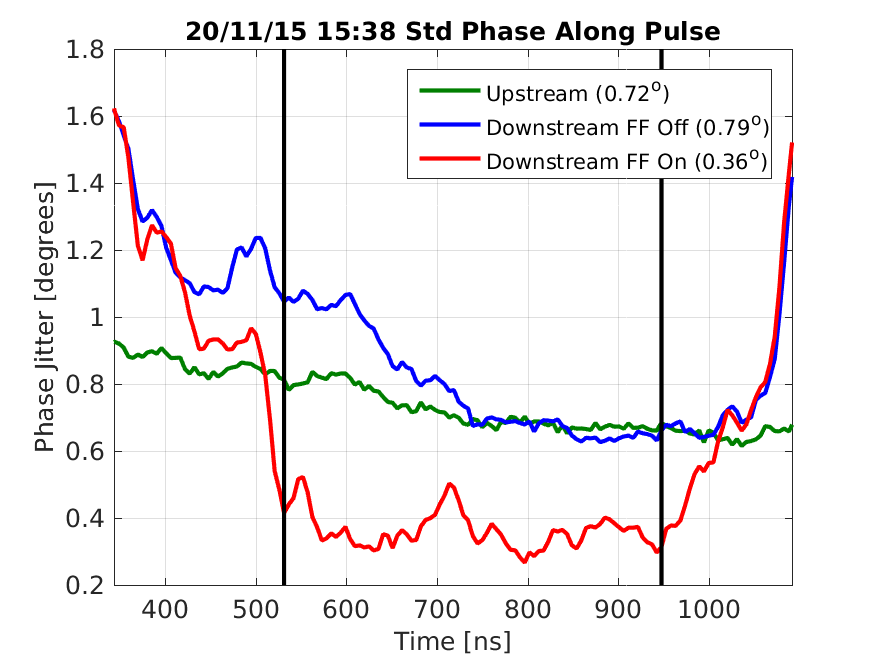
\includegraphics[width=0.75\textwidth]{Figures/feedforward/BestFF_StdPhaseAlong}
  \caption{Std phase along.}
  \label{f:BestFF_StdPhaseAlong}
\end{figure}

\begin{figure}
  \centering
  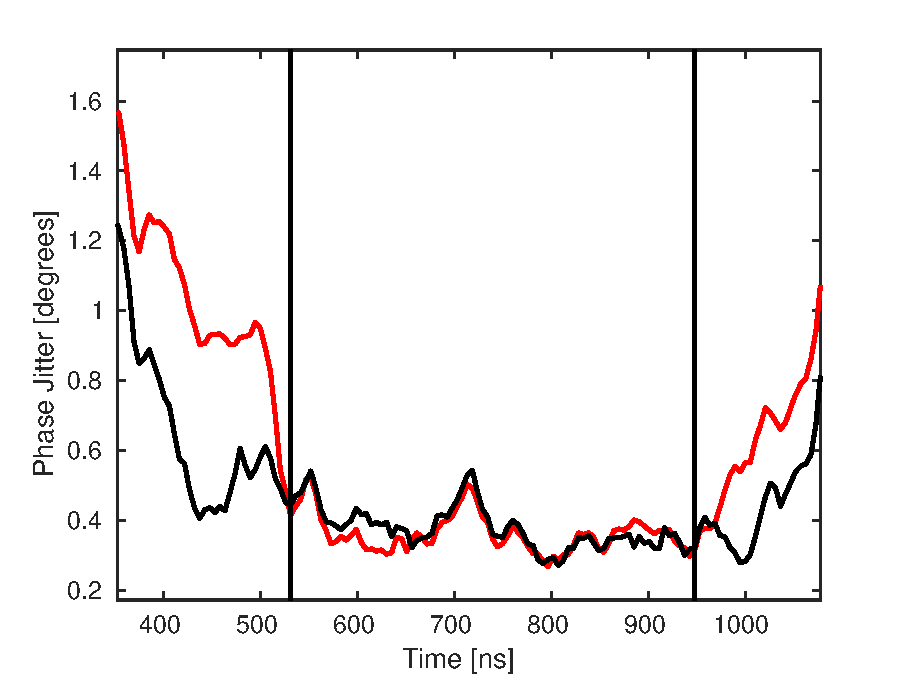
\includegraphics[width=0.75\textwidth]{Figures/feedforward/BestFF_SimStdAlongPulse}
  \caption{Std phase along.}
  \label{f:BestFF_SimStdPhaseAlong}
\end{figure}

\newsection{longPFF}{Correction on Longer Time Scales}

The remainder of this chapter focuses on remaining operational issues for the PFF system largely resulting from drifts in the CTF3 beam conditions. This section therefore discusses the status of the correction across longer time scales, presenting both the level of corrected phase jitter that can currently be achieved routinely and to highlight areas where improvements are still needed both in the PFF setup itself and the beam conditions. Being able to regularly demonstrate and maintain corrected downstream phase jitters at the level achieved in the best dataset shown previously (below \(0.3^\circ\)) on the mean phase, is one of the key goals for the PFF prototype in 2016. To be concise this section focuses on the mean phase jitter, though exactly the same arguments can be applied to the correction of the jitter along the pulse and the pulse shape.

The data used is from around 15:25 to 18:05 on the 20th November 2015, the same day as the record result previously shown which was taken during this period at 15:38. The PFF system was not operated continuously throughout this two and a half hour window but 15 individual datasets of a few hundred pulses each were taken and these results have been combined to create a large sample of 3083 interleaved pulses (1541 with the correction on and 1542 with the correction off). The raw history of the mean phases upstream and downstream with the correction on and off in the combined data are shown in Figure \ref{f:longFF_noMeanSubHistory}. The time span of each individual dataset is marked by vertical black lines and the times displayed on the plot represent the start time of each dataset. Note that the large jump in the downstream phase between the 16:00 and 16:04 datasets was caused by changes made to magnetic correctors in the TL2 chicane in order to re-optimise the beam orbit and transmission to the downstream phase monitors at this time. In Figure \ref{f:longFF_histDownstreamPhase} the mean phase is subtracted (separately for the upstream, downstream PFF off and downstream PFF on phase) from each dataset to remove this effect, making a comparison between datasets easier. It is important to emphasise that, apart from this jump in the downstream phase, the overall picture is a fair reflection of the (uncorrected) phase stability at CTF3 in optimal conditions. 

\begin{landscape}

\begin{figure}
  \centering
  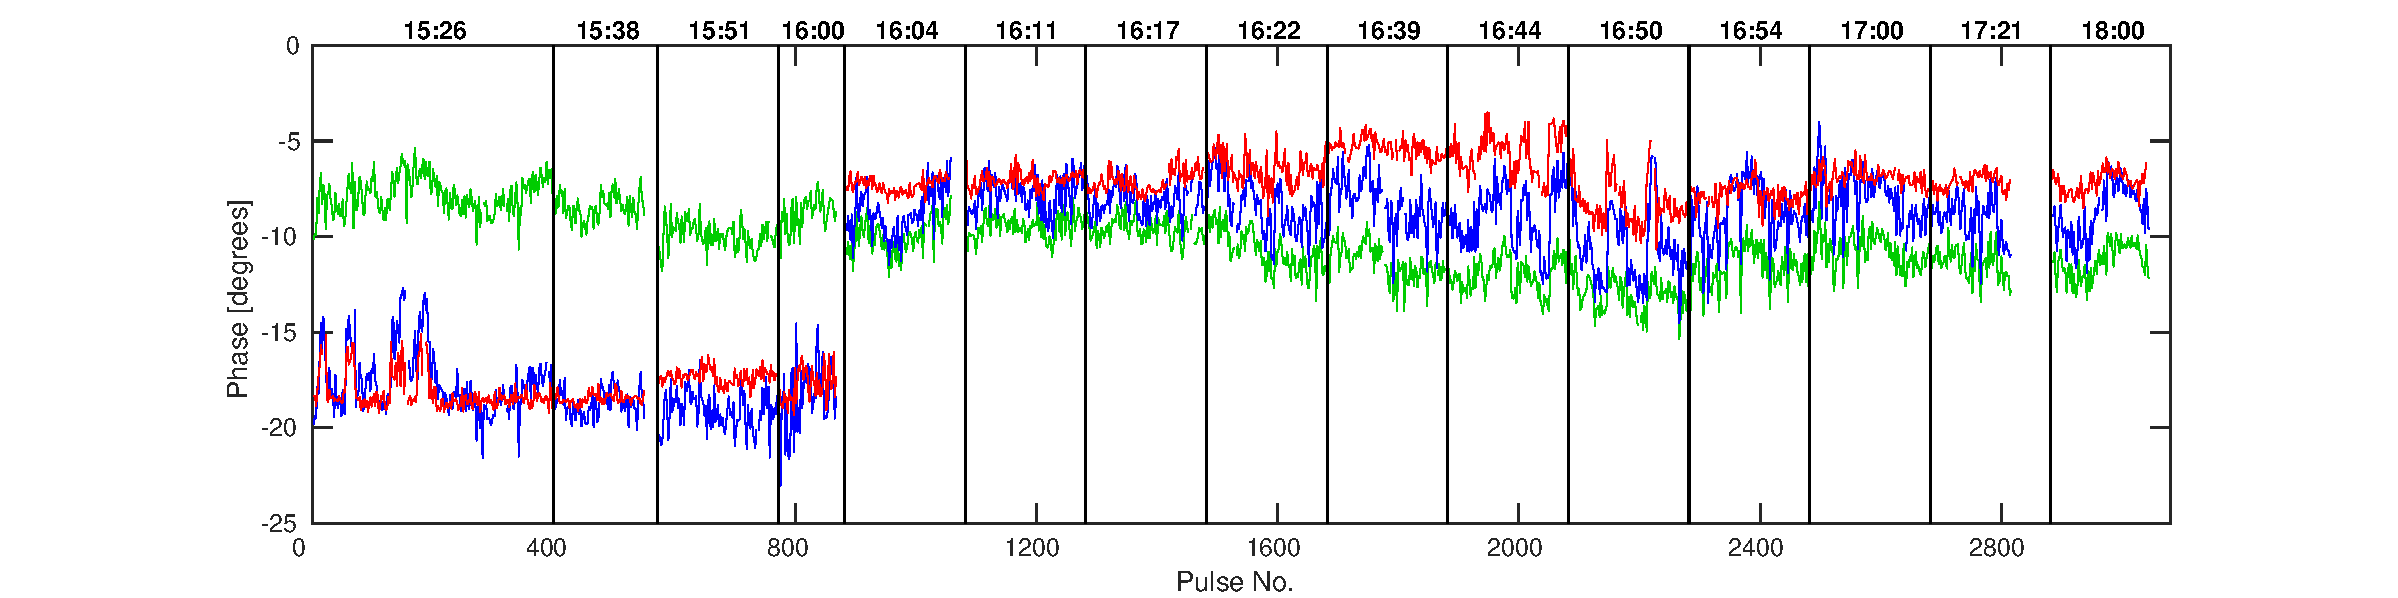
\includegraphics[width=\hsize]{Figures/feedforward/longFF_noMeanSubHistory}
  \caption{History of mean phase across datasets.}
  \label{f:longFF_noMeanSubHistory}
\end{figure}


\begin{figure}
  \centering
  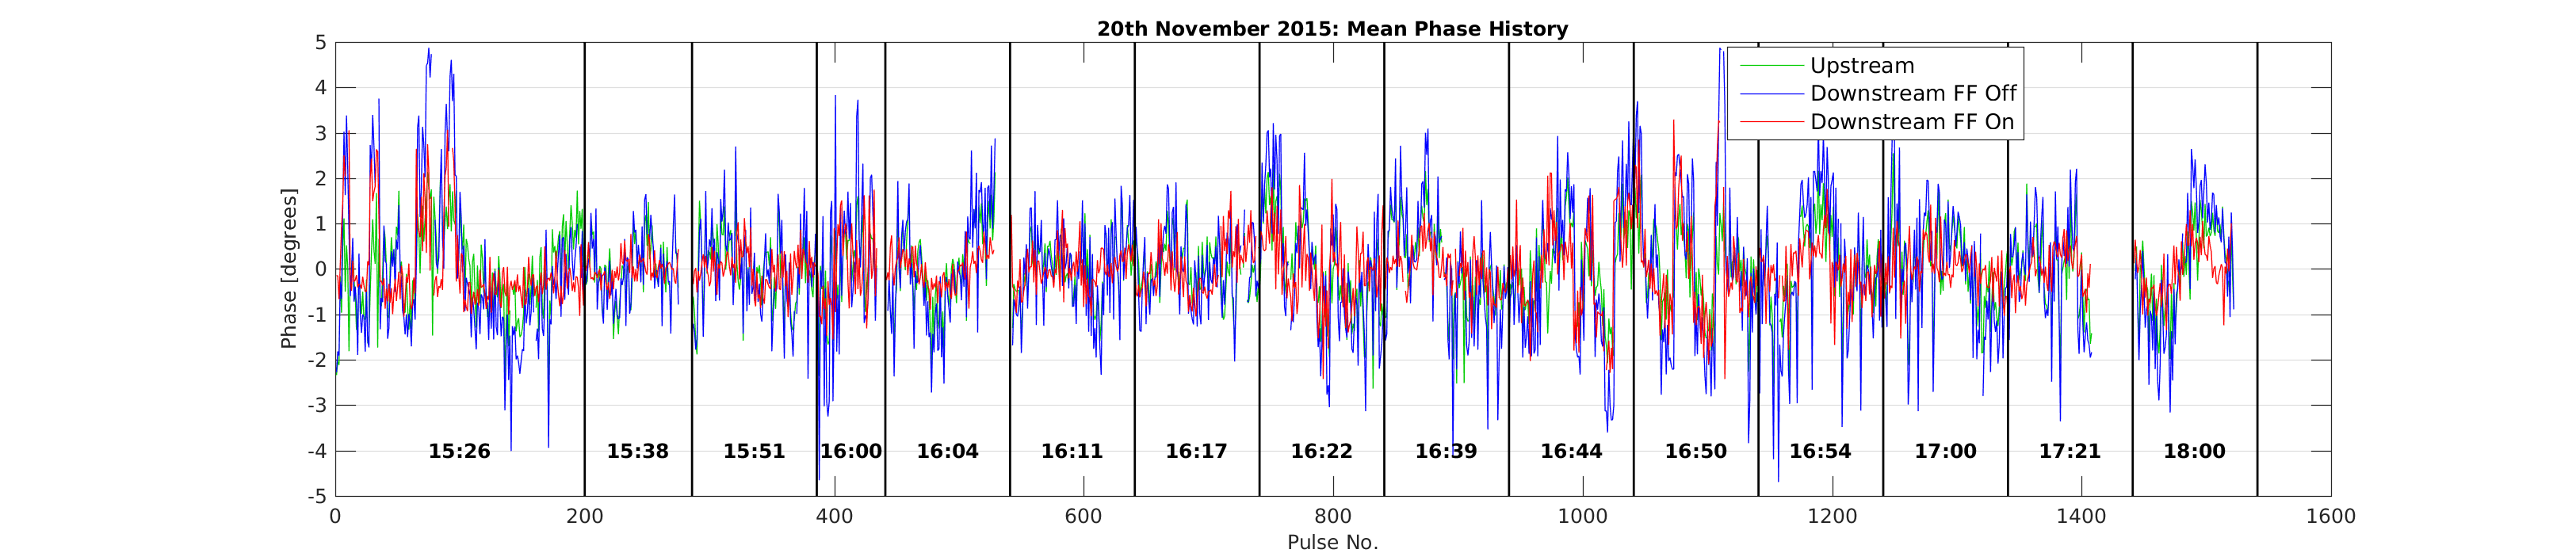
\includegraphics[width=\hsize]{Figures/feedforward/longFF_history}
  \caption{History of mean phase across datasets, with mean subtraction.}
  \label{f:longFF_history}
\end{figure}

\end{landscape}

\subsection{Upstream Phase Drifts}
\label{ss:longFF_upDrifts}

Over the course of the data taking period the mean upstream phase, in green, varies by ten degrees peak-to-peak or \(1.75 \pm 0.02^\circ\) in terms of jitter (Figure \ref{f:longFF_noMeanSubHistory}). Small drifts of up to a few degrees in the upstream phase are not an issue for the performance of the PFF correction providing the correlation between the upstream and downstream phase is not degraded. In some cases upstream phase drifts may lead to a loss in correlation, this could be the case if the source of the drift is a variation in beam energy due to the issues discussed in Chapter \ref{c:phasePropagation}, for example. The variation of the correlation between datasets is discussed later in this section.

Larger changes in the upstream phase such as the ten degree fluctuation seen here may also impact the PFF performance purely via the limited correction range of \(\pm6^\circ\) combined with the phase sag along the CTF pulse. Indeed the PFF prototype's main purpose is not to remove any large, slow phase drifts but rather the faster pulse-to-pulse jitter and high frequency variations along the pulse. The phase offset applied by the PFF correction at each sample along the downstream phase, \(\Delta\phi_d(t)\), is given by:

\begin{eqnarray}
	\Delta\phi_d(t) = \begin{cases}
	-6^\circ, &  \text{if $g\phi_u(t) \geq+6^\circ$.}\\
	+6^\circ, &  \text{if $g\phi_u(t)\leq-6^\circ$}.\\
	-g\phi_u(t), &  \text{otherwise.}
	\end{cases}
	\label{e:limCorrection}
\end{eqnarray}

Where \(\phi_u(t)\) is the upstream phase at each sample point and \(g\) is the gain factor used. As the optimal gain (Section\ref{ss:theoryGain}) for the correction is typically larger than one due to the slight amplification in the downstream phase jitter with respect to the upstream jitter the range of the PFF system in terms of the upstream phase is less than \(\pm6^\circ\) (for example \(\pm5.3^\circ\) for the 15:38 jitter record dataset with a gain of 1.13). Any point along the upstream phase with \(|g\phi_u(t)| > 6^\circ\) receives the maximum \(6^\circ\) phase shift downstream but can not be corrected to zero, with this remaining residual degrading the corrected phase jitter that can be achieved. Samples with  \(|g\phi_u(t)| > 5^\circ\) will also receive a slightly non-optimal correction due to the effects of the amplifier entering saturation, shown in Section \ref{ss:kickLin}, although this effect is assumed to be small and is not yet considered in the discussion here. 

Figure \ref{f:longFF_fractInRange} shows the fraction of pulses for which the optimal correction is within the correction range in the combined dataset. During the setup of the PFF system it is necessary to choose the zero point for the correction, i.e. the incoming upstream phase at which the correction output to the kickers is 0~V. This is done in the PFF firmware on the FONT5a board by varying a channel offset applied to the raw digitiser data from the ADC to which the upstream phase monitor mixer signal is connected [REF]. In terms of equation \ref{e:limCorrection} this is equivalent to adding a constant offset to \(\phi_u\) across the full pulse length. The optimal channel offset zeroes the mean phase (ADC output) taken across the part of the pulse where the best correction is desired (usually the flatter central part of the pulse at CTF3). In this case the effects of limited correction range are minimised, as the full \(\pm6^\circ\) range can be used to remove variations about the mean phase, rather than also having to remove a static phase offset in the overall mean. In this case the ideal correction across a 310~ns portion of the pulse is within the \(\pm6^\circ\) range 96\% of the time. 

\begin{figure}
  \centering
  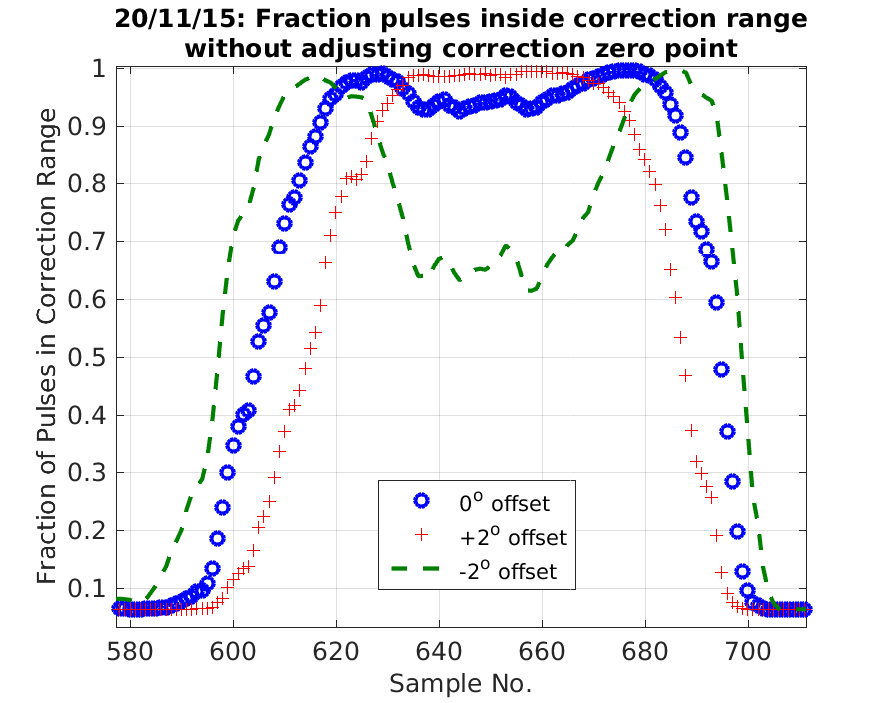
\includegraphics[width=0.75\textwidth]{Figures/feedforward/longFF_fractInRange}
  \caption{Fraction of pulses outside the correction range along the pulse.}
  \label{f:longFF_fractInRange}
\end{figure}

However, as to date this offset has been set up manually small deviations from the ideal case are possible. Figure \ref{f:longFF_fractInRange} also shows the fraction of pulses within the correction range if there is a static two degree offset in the upstream phase. In this case as many as 39\% of pulses are outside the correction range within the normally correctable central region of the pulse. To mitigate these effects and to get the largest reduction in jitter possible within each individual dataset the centring of the upstream phase in the correction range on the FONT5a board is normally adjusted between datasets. As a consequence of this differences in the upstream phase between datasets are not removed in the corrected downstream phase, as the zero point for the PFF correction is effectively moving with the phase drifts during the data taking period. These remaining slow drifts could be removed at CTF3 using a secondary ``slow phase feedback", also utilising the TL2 chicane, which is the focus of Section \ref{s:slowCorr}.

The accuracy to which the channel offset for the upstream phase has been set can be inferred by comparing the mean downstream phase in each dataset with the correction on (red) and off (blue) in Figure \ref{f:longFF_noMeanSubHistory}. In the ideal case the mean phase should be identical with the PFF system on and off, so that the full correction range is being used to correct jitter about the mean as mentioned previously. Although this is the case for some datasets, such as the 15:38 dataset, a clear offset between the two is often present, most visible in the datasets between 16:39 and 16:50 in which the corrected phase is clearly shifted several degrees with respect to the uncorrected phase. The offset in each dataset is plotted in Figure \ref{f:longFF_phaseOffset} [TODO: Change to table?]. In the region between 16:39 and 16:50 the offset falls below \(-3^\circ\). The mean offset across the combined dataset is \(-1.4^\circ\) [TODO: Calc error, weight by datset lengths]. In the following sections it will be shown that the effect of the non-optimal set point for the offset is small overall, although there is a noticeable degradation in the jitter that can be achieved in the datasets with the largest offsets. In any case, implementing an automatic procedure to set the zero point for the correction optimally in the FONT5a DAQ would be a useful improvement to the PFF setup procedure and this will be pursued for future PFF attempts in 2016.

\begin{figure}
  \centering
  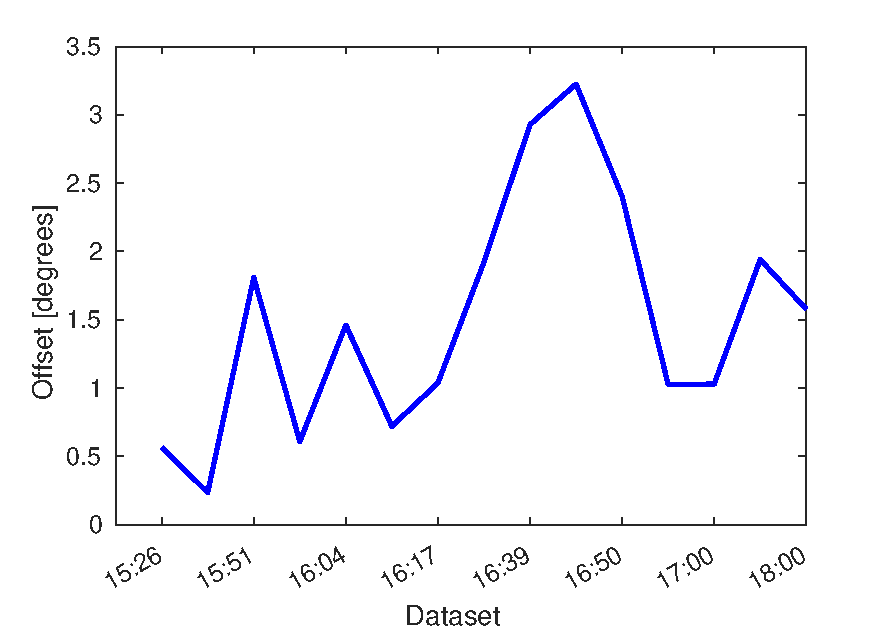
\includegraphics[width=0.75\textwidth]{Figures/feedforward/longFF_phaseOffset}
  \caption{Offset between downstream phase with FF off and FF on.}
  \label{f:longFF_phaseOffset}
\end{figure}


\subsection{Gain Stability}
\label{ss:longFF_gain}

Another PFF parameter that has been set up largely empirically to date is the correction gain. Historically, the gain set point for the PFF prototype has been determined by a combination of viewing the results of gain scans (Section \ref{s:gainScans}) and by observing the flatness of the corrected downstream phase in online displays of the phase monitor signals. If the applied gain is too large this can be quickly seen in the online monitors as the PFF system will act to invert the original phase sag along the pulse, for example. In this way it is relatively simple to find approximately the correct gain set point and further fine-tuning is done by varying the gain in small steps between datasets. In later PFF attempts this approach was complimented by implementing an online display of the optimal gain given the current measured upstream and downstream phase jitters and correlation (Section \ref{ss:sisSetup}), although this only gives a representative value when the PFF system is turned off (otherwise the calculated gain value is based on the corrected jitters and correlation). However, in this section it will be shown that due to drifts in the beam conditions at CTF3 there are large variations in the optimal gain between datasets, and these variations are rarely accurately followed in the PFF setup when using this empirical approach. An automatic gain optimisation procedure is therefore another area of improvement for future PFF attempts. Particularly if the gain was automatically updated in real time during long datasets a significant reduction in jitter could be achieved, as will be seen in the remainder of this chapter. Of course, in the ideal case the stability of beam conditions at CTF3 would be improved so that the variations in optimal gain over the course of a few hours are much smaller than those shown here.

The optimal gain depends on the downstream-upstream phase jitter ratio and the downstream-upstream phase correlation (Section \ref{ss:theoryGain}). In Figures \ref{f:longFF_noMeanSubHistory} and \ref{f:longFF_history} large differences in the phase stability in each dataset are clearly visible, comparing for example the large phase jumps in the 15:26 and 16:50 datasets to the comparatively calm periods at 15:38 and 16:17. This is summarised in Figure \ref{f:longFF_jitFFOff}, which shows the upstream and downstream (with PFF off) phase jitter across the 5--10 minute time period of each dataset. Over the course of the data taking period the mean upstream and downstream phase jitter both vary by around a factor two --- the upstream jitter between \(0.6\pm^\circ\) in the 16:17 dataset and \(1.1\pm^\circ\) at 16:22, and the downstream jitter between \(0.7\pm^\circ\) at 15:38 and \(2.2\pm^\circ\) at 16:50. [TODO: error] Given the same correlation, a factor two increase in the uncorrected downstream jitter also doubles the corrected downstream phase jitter that can be achieved with the PFF system. [TODO: explain why double jitter means double corrected jitter/refer back to prev sec].

Also of key importance for the PFF correction is that not only are there large variations in jitter between datasets but additionally in the downstream-upstream jitter ratio (dashed line in Figure \ref{f:longFF_jitFFOff}). In fact, the only dataset in which the upstream and downstream jitter are comparable is the record 15:38 dataset (with a ratio of 1.1). In all other datasets the downstream jitter is more than 1.3 times larger than the upstream jitter, reaching a maximum amplification of 2.2 in the 16:50 dataset. The mean ratio across the 15 datasets is 1.5 with a standard deviation of 0.3. [TODO: errors]

\begin{figure}
  \centering
  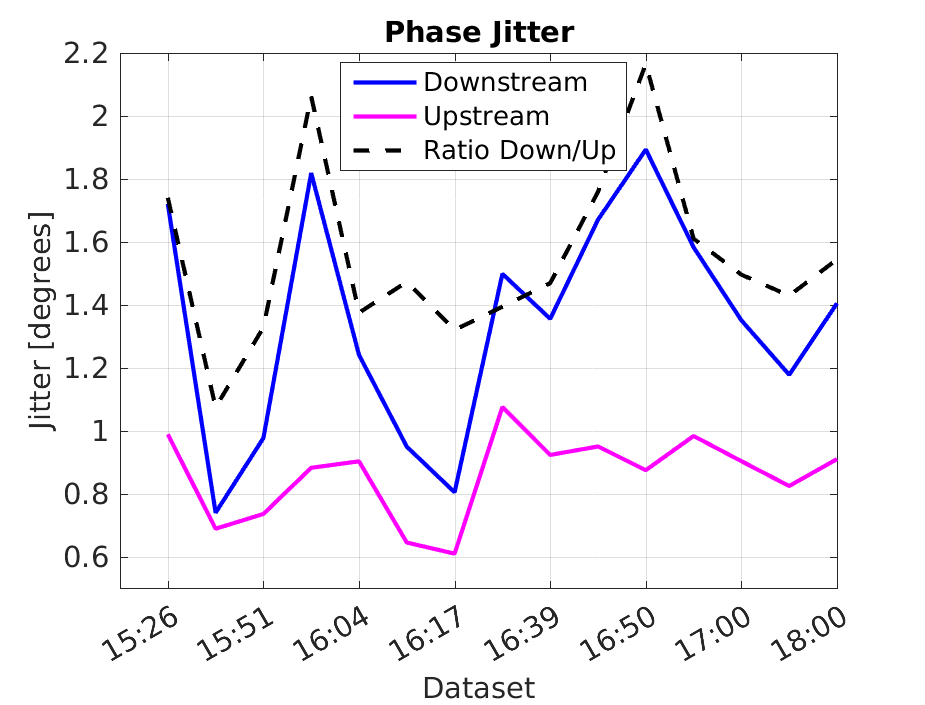
\includegraphics[width=0.75\textwidth]{Figures/feedforward/longFF_jitDatSetFFOff}
  \caption{Upstream and downstream phase jitter in each data set.}
  \label{f:longFF_jitFFOff}
\end{figure}

As well as the jitter ratio, the upstream-downstream phase correlation also varies between datasets, as shown in Figure \ref{f:longFF_corrFFOff}. The worst correlation is \(0.80\pm0.04\) in the 15:26 dataset and the best \(0.96\pm0.03\) in the 16:54 dataset. Although this has a much smaller 20\% effect on the optimal gain than the factor 2 variation in jitter ratio, it has a large effect on the theoretical jitter improvement that can be achieved with the PFF system due to the dependence on the correlation squared in Equation \ref{e:theoretJitOptGain}. With 80\% phase correlation only a theoretical factor 1.7 reduction in the downstream phase jitter can be achieved, whereas with 96\% correlation this is increased to a factor 3.6. 

\begin{figure}
  \centering
  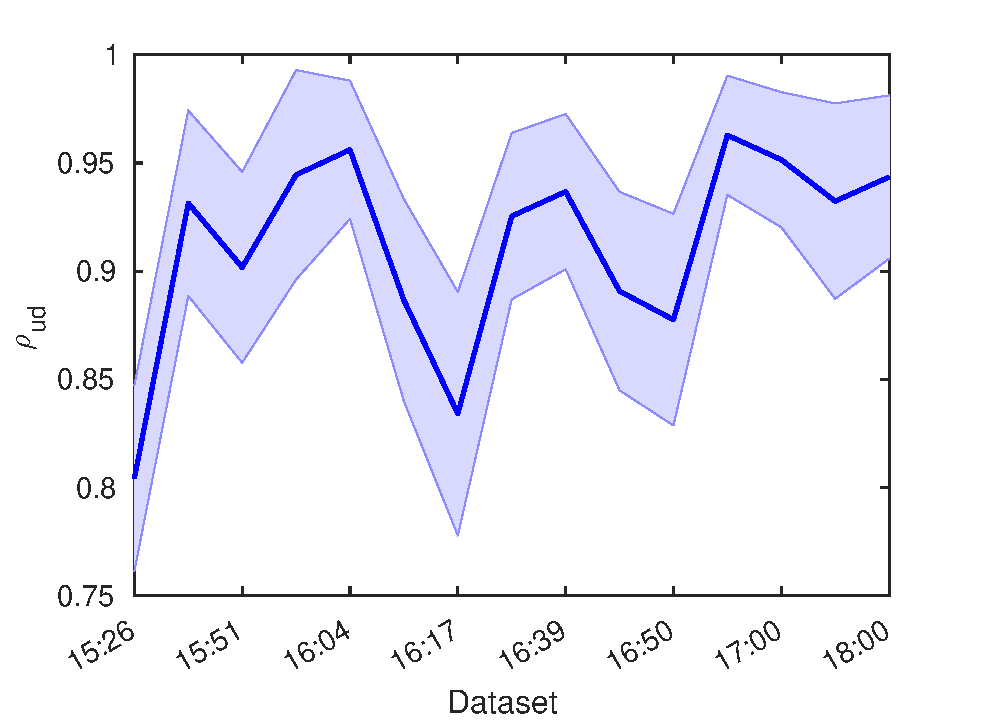
\includegraphics[width=0.75\textwidth]{Figures/feedforward/longFF_corrFFOff}
  \caption{Upstream-downstream mean phase correlation in each dataset with PFF off.}
  \label{f:longFF_corrFFOff}
\end{figure}

There is no observed dependence of the phase jitter ratio on the phase correlation, as shown in Figure \ref{f:longFF_corrVsJitRat}, so the effects of varying correlation and jitter ratio on the optimal gain are independent. [TODO:why?]. They combine to give the optimal gain plotted in Figure \ref{f:longFF_gain} (red line). As it is dominated by the differences in jitter ratio, the gain also varies by close to a factor two, varying from 1.00 in the 15:38 dataset to 1.95 in the 16:00 dataset. The real gain factor that was actually used in the dataset is also plotted, in blue. Although in places the empirically derived gain that was used follows the trend of the optimal gain, the changes are much smaller and it is clear that the real gain was systematically lower than the optimal gain. The smallest gain actually used was 1.06 (at 15:51) and the largest 1.34 (15:26 and 16:00), with an overall mean across the data taking period of 1.16 compared to the optimal value of 1.41. The impact of the real system generally under-correcting the downstream phase as a result of lower than optimal gain is discussed in the next sections.  

\begin{figure}
  \centering
  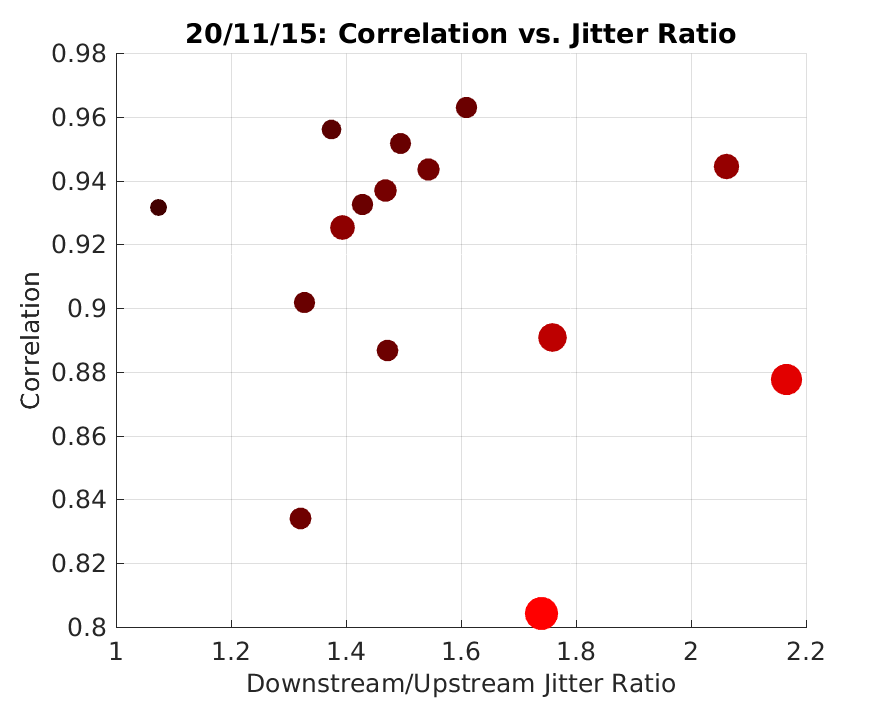
\includegraphics[width=0.75\textwidth]{Figures/feedforward/longFF_corrVsJitRat}
  \caption{Correlation vs. phase jitter ratio.}
  \label{f:longFF_corrVsJitRat}
\end{figure}

\begin{figure}
  \centering
  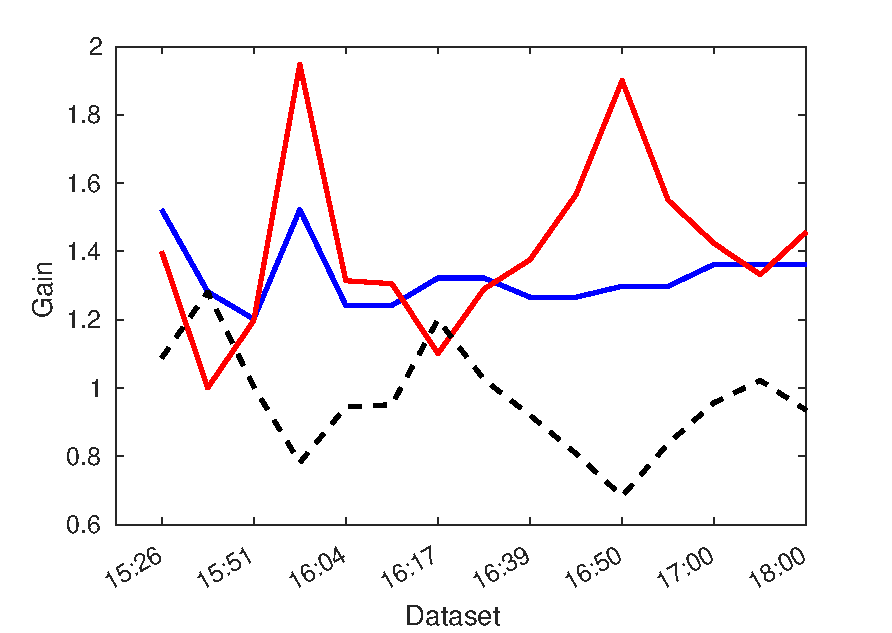
\includegraphics[width=0.75\textwidth]{Figures/feedforward/longFF_gain}
  \caption{Gain used in each dataset compared to the optimal gain.}
  \label{f:longFF_gain}
\end{figure}



\subsection{Results}
\label{ss:longFF_singleResults}

It has been shown that the frequent drifts in both phase and downstream-upstream phase jitter ratio have not been optimally taken in to account in the PFF setup in terms of the used offset and gain. Nevertheless, even with a sub-optimal setup a large reduction in the downstream phase jitter can be achieved in all datasets. In the remainder of this section it will be shown that considering these constraints the PFF system is achieving close to peak performance, as well as highlighting the benefit that more accurate gain and offset control would have.

Firstly referring back to Figure \ref{f:longFF_corrVsJitRat}, the size (area) and colour of the markers in the plot depend on the corrected downstream jitter that could be achieved in that dataset using the optimal gain. Small, black markers correspond to the lowest theoretical jitter and large, red markers to the largest theoretical jitter. This is to emphasise again that it is a compromise between high correlation and low initial downstream jitter (and by extension low downstream-upstream jitter ratio) that gives the best conditions for the PFF correction. There are seven datasets with an achieved correlation of above the 93\% seen in the 15:38 record result, for example, but they yield worse theoretical corrections as 15:38 remains the only dataset in which a high correlation and low upstream-downstream jitter amplification have been achieved at the same time.

Figure \ref{f:longFF_datSetJitSim} and Table \ref{t:LongFFIndivSim} then show the simulated corrected downstream jitter chronologically for each dataset with five different simulation setups:
\begin{itemize}
\item \textbf{Unlimited:} With unlimited correction range and the optimal gain (theoretical limit).
\item \textbf{6deg Range:} With \(\pm6^\circ\) correction range and the optimal gain.
\item \textbf{Real Gain:} With \(\pm6^\circ\) correction range and the real gain used by the actual PFF system.
\item \textbf{Real Offset:} With \(\pm6^\circ\) correction range and the real offset in the actual PFF setup.
\item \textbf{All effects:} With \(\pm6^\circ\) correction range, the real gain, and the real offset in the actual PFF setup.
\end{itemize}

[TODO: Simulations should use 5.5 degree range instead AND I used FONT gain conversion factor of 711 but correct value is 624]

By comparing the results of these five simulations it is possible to identify which PFF parameters are most critical for the correction performance. Later, by comparing the most restricted simulation, including the real offset and gain, to the phase jitter actually achieved it can be determined whether the PFF system is behaving as expected or whether there are remaining effects that need to be understood.

With the ideal PFF setup the \(\pm6^\circ\) range set by the amplifier power is sufficient to be able to optimally correct almost all the natural phase jitter, thus the difference between the unlimited and 6deg range simulation is small. The only visible effect is in datasets with the largest incoming phase jitter, with a maximal \(0.05^o\) degradation in the achievable phase jitter in the 16:00 dataset with an incoming uncorrected phase jitter of 1.8 degrees, for example. The correction range is therefore not a limiting factor for the PFF performance in normal conditions, although it may become significant if the PFF system were operated on longer time scales without updating the offset or when trying to demonstrate a factor 10 reduction in jitter (Section \ref{s:pffNovelSetups}).

Depending on the dataset, the effects of using non-optimal gain and non-optimal offset are much larger. In the 15:26, 15:38, 15:51 and 16:17 datasets where both the gain and offset are close to optimal all five simulations give close to the same result, as expected. For most the other datasets the largest effect on the achievable corrected jitter comes from the non-optimal gain, with a difference of up to \(0.24^\circ\) in the simulated phase jitter (16:00). However, in the period between 16:22 and 16:50 where the offset in the PFF setup was largest its influence can be similar to that of the non-optimal gain, or in some cases larger, with a maximal degradation in the achievable downstream jitter of \(0.16^\circ\) (16:50) coming from the offset alone. With the effects of limited correction range, non-optimal offset and non-optimal gain combined the achieved corrected jitter is expected to be up to \(0.29^\circ\) worse than the theoretical limit (16:50), although in most datasets the effect is much smaller than this, with no significant difference between the unlimited and all effects simulations in the previously mentioned 15:26, 15:38, 15:51 and 16:17 datasets, for example. 

Only the 15:38 dataset has a theoretical (and in all simulation scenarios) corrected downstream jitter of below \(0.3^\circ\) but in 10 out of 15 datasets below \(0.5^\circ\) jitter could have been achieved with an optimal PFF setup (or in 6 out of 15 with the actual setup). Further improvements not only in the peak phase propagation conditions achieved so far but also clearly on the stability of the phase propagation are therefore needed to demonstrate CLIC level phase stability both on short and long time scales at CTF3.

\begin{figure}
  \centering
  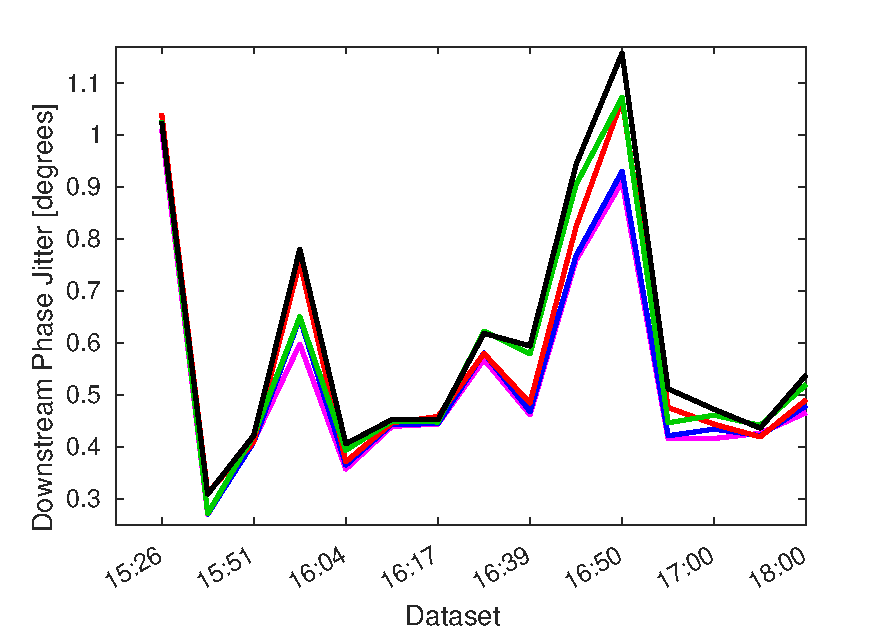
\includegraphics[width=0.75\textwidth]{Figures/feedforward/longFF_datSetJitSim}
  \caption{Theoretical corrected downstream jitter with optimal and used gain.}
  \label{f:longFF_datSetJitSim}
\end{figure}

The achieved downstream jitter with the actual PFF system are presented in Figure \ref{f:longFF_jitDatSet} and Table \ref{t:LongFFIndiv}, along with the uncorrected downstream and upstream jitter and the most realistic "all effects" simulation of the expected performance. Overall the agreement between the downstream jitter achieved with the actual PFF system and the simulation is very good. This gives confidence that the PFF system is behaving as expected and all the effects limiting the current performance are understood and in principle can be improved to yield lower jitter in future PFF attempts. However, there is a region between 16:17 and 16:44 where differences between the simulation and actual system can be seen. In particular, the \(0.58\pm0.04^\circ\) and \(0.82\pm0.06^\circ\) downstream jitter in the 16:17 and 16:22 datasets, respectively, are noticeably worse than the simulated results of \(0.45\pm0.03\) and \(0.65\pm0.05\). The source of this is not yet understood and possibly hints at additional areas for improvement in the PFF setup. 

Nevertheless, despite highlighting where the PFF setup and beam conditions are non-optimal during this discussion the overall benefit of the PFF system is clear - the downstream phase jitter is reduced in every dataset, with a maximum reduction factor of 3.2 in the 16:05 dataset (in which the highest correlation of 96\% was achieved). Attempts to demonstrate a larger reduction factor, closer to the CLIC specification of an order of magnitude, are presented in Section \ref{s:pffNovelSetups}. 

\begin{figure}
  \centering
  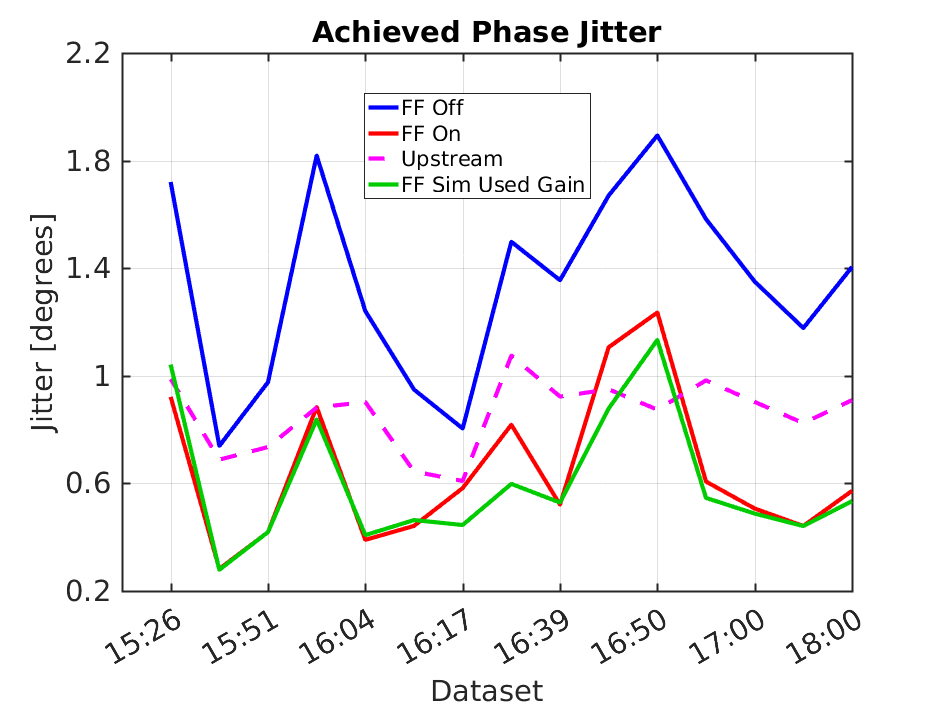
\includegraphics[width=0.75\textwidth]{Figures/feedforward/longFF_jitDatSet}
  \caption{Corrected downstream jitter with the actual PFF system.}
  \label{f:longFF_jitDatSet}
\end{figure}

\begin{table}
  \begin{center}
    \begin{tabular}{ c  c  c  c  c  c  }
	   \hline
       Time & Unlimited &  6deg Range &  Real Gain &  Real Offset &  All Effects \\ \hline
15:26 & \(1.01\pm0.05^\circ\) & \(1.04\pm0.05^\circ\) & \(1.04\pm0.05\) & \(1.03\pm0.05^\circ\) & \(1.03\pm0.05^\circ\) \\
15:38 & \(0.27\pm0.02^\circ\) & \(0.27\pm0.02^\circ\) & \(0.28\pm0.02\) & \(0.27\pm0.02^\circ\) & \(0.28\pm0.02^\circ\) \\
15:51 & \(0.41\pm0.03^\circ\) & \(0.41\pm0.03^\circ\) & \(0.42\pm0.03\) & \(0.42\pm0.03^\circ\) & \(0.44\pm0.03^\circ\) \\
16:00 & \(0.60\pm0.06^\circ\) & \(0.65\pm0.07^\circ\) & \(0.84\pm0.09\) & \(0.65\pm0.07^\circ\) & \(0.86\pm0.09^\circ\) \\
16:04 & \(0.36\pm0.03^\circ\) & \(0.36\pm0.03^\circ\) & \(0.41\pm0.03\) & \(0.39\pm0.03^\circ\) & \(0.44\pm0.03^\circ\) \\
16:11 & \(0.44\pm0.03^\circ\) & \(0.44\pm0.03^\circ\) & \(0.46\pm0.03\) & \(0.45\pm0.03^\circ\) & \(0.47\pm0.03^\circ\) \\
16:17 & \(0.44\pm0.03^\circ\) & \(0.44\pm0.03^\circ\) & \(0.45\pm0.03\) & \(0.45\pm0.03^\circ\) & \(0.45\pm0.03^\circ\) \\
16:22 & \(0.57\pm0.04^\circ\) & \(0.58\pm0.04^\circ\) & \(0.60\pm0.04\) & \(0.62\pm0.04^\circ\) & \(0.65\pm0.05^\circ\) \\
16:39 & \(0.46\pm0.03^\circ\) & \(0.47\pm0.03^\circ\) & \(0.53\pm0.04\) & \(0.58\pm0.04^\circ\) & \(0.62\pm0.04^\circ\) \\
16:44 & \(0.76\pm0.05^\circ\) & \(0.77\pm0.05^\circ\) & \(0.88\pm0.06\) & \(0.90\pm0.06^\circ\) & \(0.98\pm0.07^\circ\) \\
16:50 & \(0.91\pm0.07^\circ\) & \(0.93\pm0.07^\circ\) & \(1.13\pm0.08\) & \(1.07\pm0.08^\circ\) & \(1.20\pm0.09^\circ\) \\
16:54 & \(0.42\pm0.03^\circ\) & \(0.42\pm0.03^\circ\) & \(0.55\pm0.04\) & \(0.45\pm0.03^\circ\) & \(0.58\pm0.04^\circ\) \\
17:00 & \(0.42\pm0.03^\circ\) & \(0.43\pm0.03^\circ\) & \(0.49\pm0.03\) & \(0.46\pm0.03^\circ\) & \(0.52\pm0.04^\circ\) \\
17:21 & \(0.43\pm0.04^\circ\) & \(0.42\pm0.04^\circ\) & \(0.44\pm0.04\) & \(0.44\pm0.04^\circ\) & \(0.47\pm0.04^\circ\) \\
18:00 & \(0.47\pm0.04^\circ\) & \(0.48\pm0.04^\circ\) & \(0.53\pm0.04\) & \(0.52\pm0.04^\circ\) & \(0.58\pm0.05^\circ\) \\
    \end{tabular}
    \caption{Simulated feedforward results from 20th November 2015.}
  	\label{t:LongFFIndivSim}
  \end{center}
\end{table}


\begin{table}
  \begin{center}
    \begin{tabular}{ c  c  c  c  c  c  }
	   \hline
	           & Up  & Down Jitter & Correlation  & Down Jitter  & Down Jitter \\
       Time & Jitter &  FF Off &  FF Off &  FF On &  Sim \\ \hline
15:26 & \(0.99\pm0.05^\circ\) & \(1.72\pm0.09^\circ\) & \(0.80\pm0.04\) & \(0.92\pm0.05^\circ\) & \(1.03\pm0.05^\circ\) \\
15:38 & \(0.57\pm0.05^\circ\) & \(0.74\pm0.06^\circ\) & \(0.93\pm0.04\) & \(0.28\pm0.02^\circ\) & \(0.28\pm0.02^\circ\) \\
15:51 & \(0.74\pm0.05^\circ\) & \(0.98\pm0.07^\circ\) & \(0.90\pm0.04\) & \(0.42\pm0.03^\circ\) & \(0.44\pm0.03^\circ\) \\
16:00 & \(0.69\pm0.07^\circ\) & \(1.82\pm0.19^\circ\) & \(0.94\pm0.05\) & \(0.88\pm0.09^\circ\) & \(0.86\pm0.09^\circ\) \\
16:04 & \(0.79\pm0.06^\circ\) & \(1.24\pm0.09^\circ\) & \(0.96\pm0.03\) & \(0.39\pm0.03^\circ\) & \(0.44\pm0.03^\circ\) \\
16:11 & \(0.70\pm0.05^\circ\) & \(0.95\pm0.07^\circ\) & \(0.89\pm0.05\) & \(0.44\pm0.03^\circ\) & \(0.47\pm0.03^\circ\) \\
16:17 & \(0.61\pm0.04^\circ\) & \(0.80\pm0.06^\circ\) & \(0.83\pm0.06\) & \(0.58\pm0.04^\circ\) & \(0.45\pm0.03^\circ\) \\
16:22 & \(0.99\pm0.07^\circ\) & \(1.50\pm0.11^\circ\) & \(0.93\pm0.04\) & \(0.82\pm0.06^\circ\) & \(0.65\pm0.05^\circ\) \\
16:39 & \(0.96\pm0.07^\circ\) & \(1.36\pm0.10^\circ\) & \(0.94\pm0.04\) & \(0.52\pm0.04^\circ\) & \(0.62\pm0.04^\circ\) \\
16:44 & \(0.84\pm0.06^\circ\) & \(1.67\pm0.12^\circ\) & \(0.89\pm0.05\) & \(1.11\pm0.08^\circ\) & \(0.98\pm0.07^\circ\) \\
16:50 & \(0.88\pm0.06^\circ\) & \(1.89\pm0.13^\circ\) & \(0.88\pm0.05\) & \(1.24\pm0.09^\circ\) & \(1.20\pm0.09^\circ\) \\
16:54 & \(1.08\pm0.08^\circ\) & \(1.58\pm0.11^\circ\) & \(0.96\pm0.03\) & \(0.61\pm0.04^\circ\) & \(0.58\pm0.04^\circ\) \\
17:00 & \(0.85\pm0.06^\circ\) & \(1.35\pm0.10^\circ\) & \(0.95\pm0.03\) & \(0.51\pm0.04^\circ\) & \(0.52\pm0.04^\circ\) \\
17:21 & \(0.84\pm0.07^\circ\) & \(1.18\pm0.10^\circ\) & \(0.93\pm0.05\) & \(0.44\pm0.04^\circ\) & \(0.47\pm0.04^\circ\) \\
18:00 & \(0.95\pm0.08^\circ\) & \(1.40\pm0.11^\circ\) & \(0.94\pm0.04\) & \(0.57\pm0.05^\circ\) & \(0.58\pm0.05^\circ\) \\
    \end{tabular}
    \caption{Feedforward results from 20th November 2015.}
  	\label{t:LongFFIndiv}
  \end{center}
\end{table}

Rather than showing each individual dataset, Figures \ref{f:longFF_histDownstreamPhase}---\ref{f:longFF_scatterFFSimReal} and Table \ref{t:LongFF} present the upstream-downstream phase distribution and overall jitter improvement with all the datasets combined. In order to yield meaningful results the mean upstream and downstream phase (both with FF on and FF off) are subtracted separately for each dataset. The effect of this can be seen by comparing Figure \ref{f:longFF_noMeanSubHistory} (with no mean subtraction) and Figure \ref{f:longFF_history}. Without this subtraction any calculated jitter and correlation values across the combined dataset would be dominated by changes in the downstream phase resulting from changing the zero point (offset) for the correction between datasets, plus the large step in the downstream phase between the 16:00 and 16:04 datasets due to a beam setup change. 

Overall, the actual system is able to reduce an initial downstream jitter of \(1.40\pm0.03^\circ\) by a factor of two, down to \(0.72\pm0.01^\circ\) (Figures \ref{f:longFF_histDownstreamPhase}, \ref{f:longFF_scatterFFOff} and \ref{f:longFF_scatterFFOn}). Due to the non-optimal setup in some datasets as shown the PFF system does not remove all correlation between the upstream and corrected downstream phase, with the initial correlation of \(0.89\pm0.01\) reduced only to \(0.48\pm0.02\). With a completely optimal setup and unlimited correction range all the correlation would be removed and the jitter could have been reduced further to \(0.61\pm0.01^\circ\) (Figure \ref{f:longFF_scatterFFSimOpt}). To achieve better than this improved beam conditions are reuired, including more stable and higher upstream-downstream phase correlation and lower and more stable phase jitters. Considering the constraints of the actual system and non-optimal setup, the achieved downstream jitter and residual correlation are as expected (Figure \ref{f:longFF_scatterFFSimReal}).

\begin{figure}
  \centering
  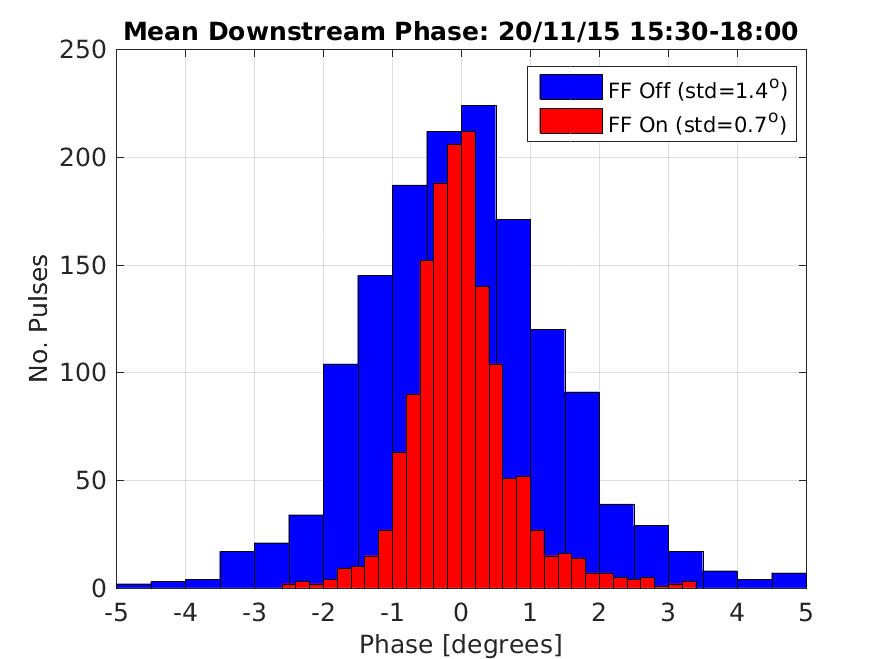
\includegraphics[width=0.75\textwidth]{Figures/feedforward/longFF_histDownstreamPhase}
  \caption{Histogram showing overall distribution of downstream phase with FF off and on.}
  \label{f:longFF_histDownstreamPhase}
\end{figure}

\begin{figure}
  \centering
  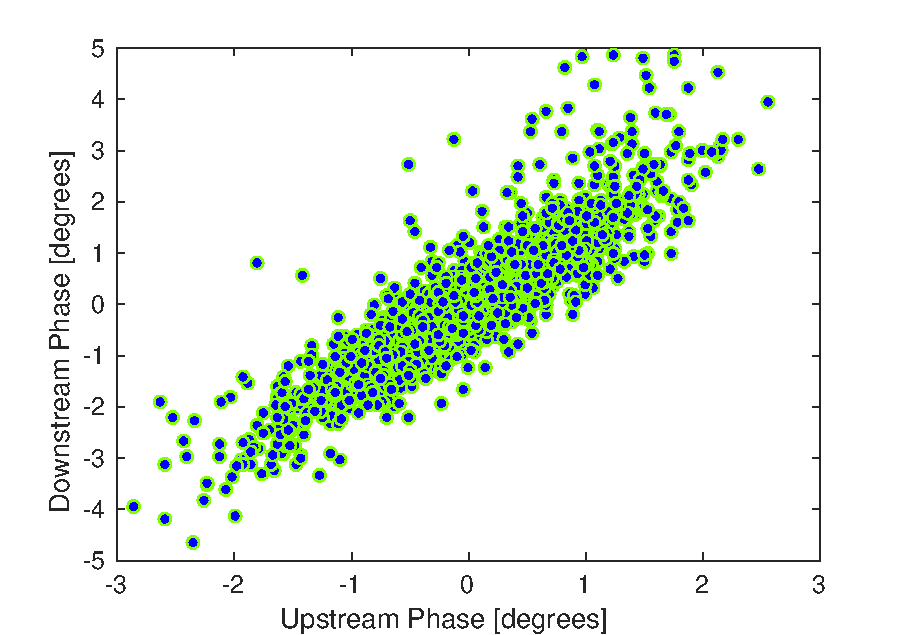
\includegraphics[width=0.75\textwidth]{Figures/feedforward/longFF_scatterFFOff}
  \caption{Downstream phase vs. upstream phase with FF off.}
  \label{f:longFF_scatterFFOff}
\end{figure}

\begin{figure}
  \centering
  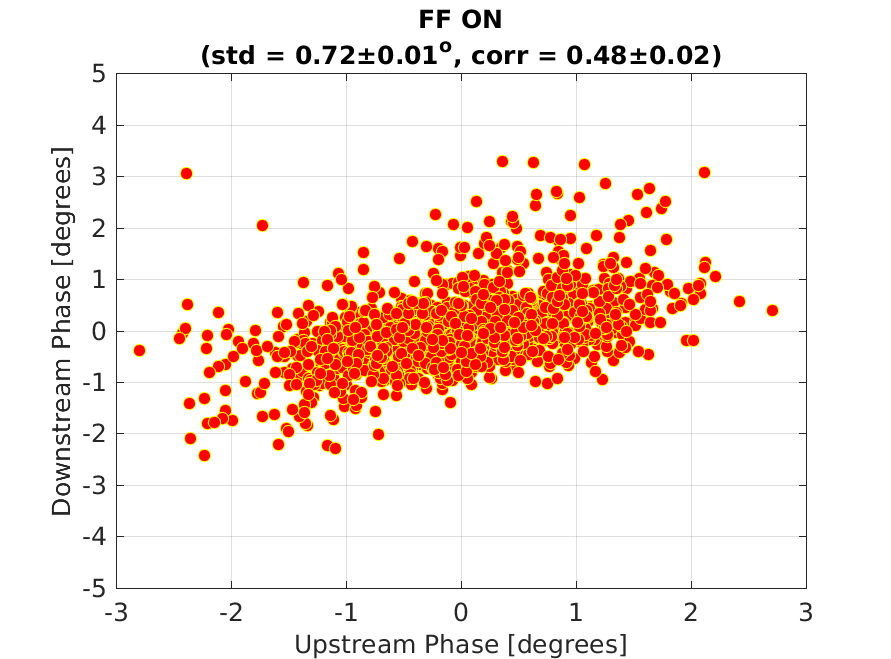
\includegraphics[width=0.75\textwidth]{Figures/feedforward/longFF_scatterFFOn}
  \caption{Downstream phase vs. upstream phase with FF on.}
  \label{f:longFF_scatterFFOn}
\end{figure}

\begin{figure}
  \centering
  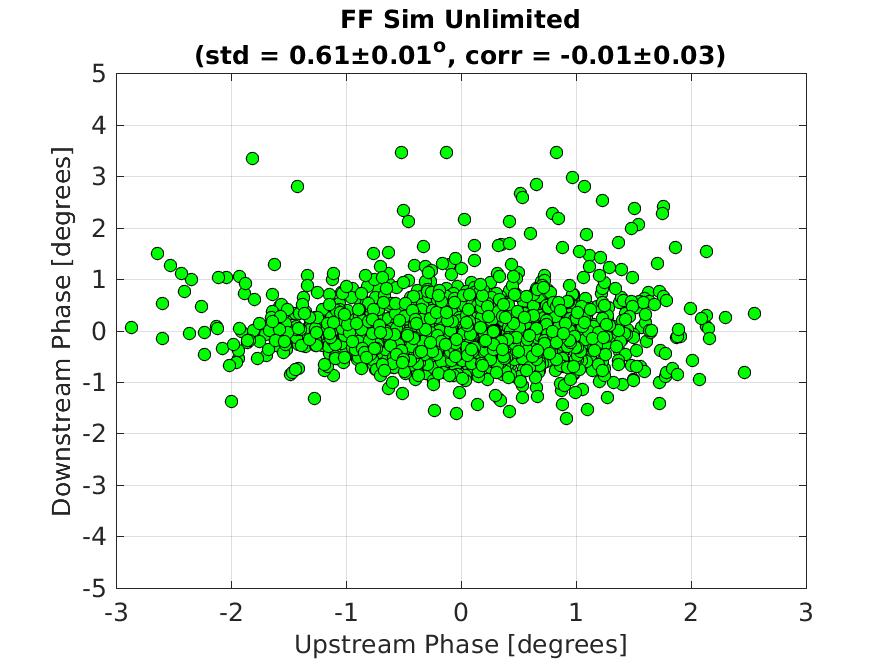
\includegraphics[width=0.75\textwidth]{Figures/feedforward/longFF_scatterFFSimOpt}
  \caption{Downstream phase vs. upstream phase with FF simulated at optimal gain.}
  \label{f:longFF_scatterFFSimOpt}
\end{figure}

\begin{figure}
  \centering
  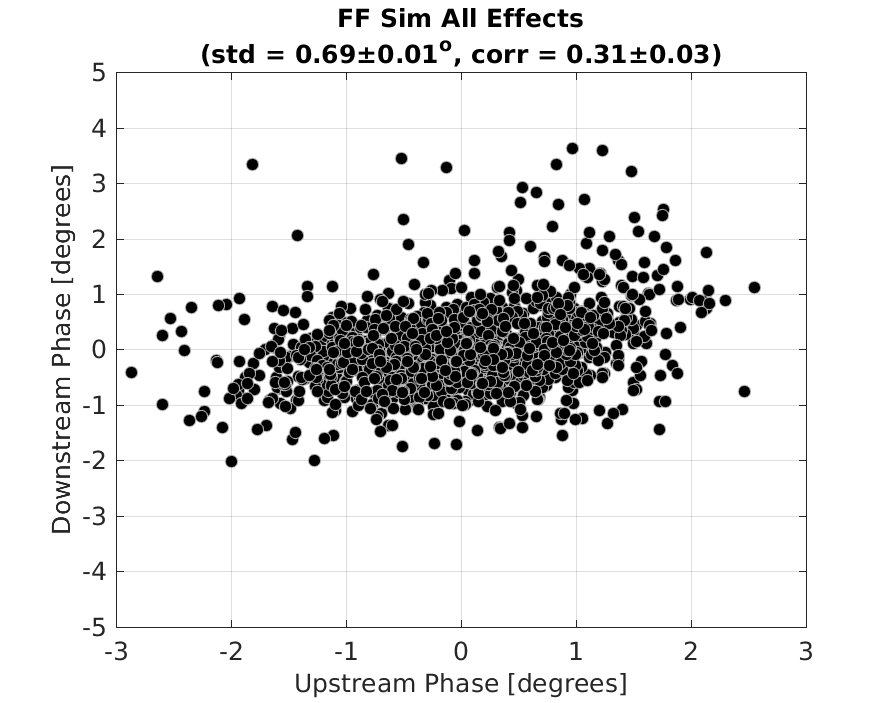
\includegraphics[width=0.75\textwidth]{Figures/feedforward/longFF_scatterFFSimReal}
  \caption{Downstream phase vs. upstream phase with FF simulated with actual gain used.}
  \label{f:longFF_scatterFFSimReal}
\end{figure}

\begin{table}
  \begin{center}
    \begin{tabular}{| c | c | c | c |}
	   \hline
       Correction Status & Upstream Jitter & Downstream Jitter & Correlation \\ \hline
       FF Off & \(0.88\pm0.02^\circ\) & \(1.40\pm0.03^\circ\) & \(0.89\pm0.01\) \\
	   FF On & \(0.86\pm0.02^\circ\) & \(0.72\pm0.01^\circ\) & \(0.48\pm0.02\) \\
	   FF Sim Opt Gain & \(0.88\pm0.02^\circ\) & \(0.61\pm0.01^\circ\) & \(-0.01\pm0.03\) \\
	   FF Sim Real Gain & \(0.88\pm0.02^\circ\) & \(0.68\pm0.01^\circ\) & \(0.35\pm0.02\) \\
	   FF Sim Offset & \(0.88\pm0.02^\circ\) & \(0.69\pm0.01^\circ\) & \(0.36\pm0.02\) \\
	   FF Sim 90\% Real Gain & \(0.88\pm0.02^\circ\) & \(0.72\pm0.01^\circ\) & \(0.46\pm0.02\) \\ \hline
    \end{tabular}
    \caption{Feedforward results using combined data from 20th November 2015. [TODO: this table shows results from old simulations!]}
  	\label{t:LongFF}
  \end{center}
\end{table}

\newsection{pffPosImprovements}{Possible Areas for Future Improvement}


